\chapter{Análisis del sistema}
\label{ch:analisis}
En este capítulo se explicará de qué es capaz el producto desarrollado. Comienza con una descripción del sistema de una manera detallada, después se extraerán los requisitos de usuario y casos de uso, que nos permiten hacernos una idea clara de lo que necesita el sistema y poder conceptualizarlo en forma de requisitos de software. En último lugar se establecerá la relación entre los requisitos de usuario y los de software en una matriz de trazabilidad, pudiendo así comprobar que todas las peticiones del usuario han sido tenidas en cuenta.

Además, este capítulo sirve como base para los siguientes, como son el de Diseño y el de Implementación, en los que, basándose en los requisitos recogidos, se empezara a dar forma al sistema.

\section{Definición del Sistema}
El propósito de este proyecto es desarrollar un dispositivo que nos proporcione videovigilancia y medidas de diferentes factores ambientales, para garantizar la seguridad de un CPD. Las diferentes medidas que se tomen se almacenaran para poder ser consultadas junto con la imagen de videovigilancia a través de una plataforma web.
\begin{figure}[H]
	\ffigbox[\FBwidth]
	{\caption{Diagrama del sistema}}
	{\tikzset{every picture/.style={line width=0.75pt}} %set default line width to 0.75pt        
	
	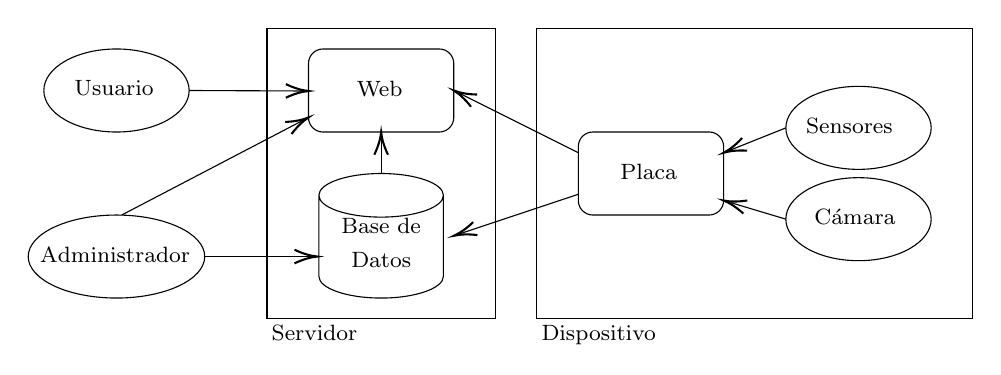
\begin{tikzpicture}[x=0.75pt,y=0.75pt,yscale=-1,xscale=1]
		
		\draw   (82.49,90) .. controls (82.49,78.95) and (98.16,70) .. (117.49,70) .. controls (136.82,70) and (152.49,78.95) .. (152.49,90) .. controls (152.49,101.05) and (136.82,110) .. (117.49,110) .. controls (98.16,110) and (82.49,101.05) .. (82.49,90) -- cycle ;
		
		\draw   (320,60) -- (530,60) -- (530,200) -- (320,200) -- cycle ;
		\draw   (440,108) .. controls (440,96.95) and (455.67,88) .. (475,88) .. controls (494.33,88) and (510,96.95) .. (510,108) .. controls (510,119.05) and (494.33,128) .. (475,128) .. controls (455.67,128) and (440,119.05) .. (440,108) -- cycle ;
		
		\draw   (275,140.5) -- (275,179.5) .. controls (275,185.3) and (261.57,190) .. (245,190) .. controls (228.43,190) and (215,185.3) .. (215,179.5) -- (215,140.5)(275,140.5) .. controls (275,146.3) and (261.57,151) .. (245,151) .. controls (228.43,151) and (215,146.3) .. (215,140.5) .. controls (215,134.7) and (228.43,130) .. (245,130) .. controls (261.57,130) and (275,134.7) .. (275,140.5) -- cycle ;
		
		\draw   (210,77) .. controls (210,73.13) and (213.13,70) .. (217,70) -- (273,70) .. controls (276.87,70) and (280,73.13) .. (280,77) -- (280,103) .. controls (280,106.87) and (276.87,110) .. (273,110) -- (217,110) .. controls (213.13,110) and (210,106.87) .. (210,103) -- cycle ;
		
		\draw   (340,117) .. controls (340,113.13) and (343.13,110) .. (347,110) -- (403,110) .. controls (406.87,110) and (410,113.13) .. (410,117) -- (410,143) .. controls (410,146.87) and (406.87,150) .. (403,150) -- (347,150) .. controls (343.13,150) and (340,146.87) .. (340,143) -- cycle ;
		
		\draw   (440,152) .. controls (440,140.95) and (455.67,132) .. (475,132) .. controls (494.33,132) and (510,140.95) .. (510,152) .. controls (510,163.05) and (494.33,172) .. (475,172) .. controls (455.67,172) and (440,163.05) .. (440,152) -- cycle ;
		
		\draw    (440,152) -- (411.92,143.57) ;
		\draw [shift={(410,143)}, rotate = 376.7] [color={rgb, 255:red, 0; green, 0; blue, 0 }  ][line width=0.75]    (10.93,-3.29) .. controls (6.95,-1.4) and (3.31,-0.3) .. (0,0) .. controls (3.31,0.3) and (6.95,1.4) .. (10.93,3.29)   ;
		\draw    (440,108) -- (411.86,119.26) ;
		\draw [shift={(410,120)}, rotate = 338.2] [color={rgb, 255:red, 0; green, 0; blue, 0 }  ][line width=0.75]    (10.93,-3.29) .. controls (6.95,-1.4) and (3.31,-0.3) .. (0,0) .. controls (3.31,0.3) and (6.95,1.4) .. (10.93,3.29)   ;
		\draw    (152.49,90) -- (208,90.24) ;
		\draw [shift={(210,90.25)}, rotate = 180.25] [color={rgb, 255:red, 0; green, 0; blue, 0 }  ][line width=0.75]    (10.93,-3.29) .. controls (6.95,-1.4) and (3.31,-0.3) .. (0,0) .. controls (3.31,0.3) and (6.95,1.4) .. (10.93,3.29)   ;
		\draw    (340,120) -- (281.79,90.89) ;
		\draw [shift={(280,90)}, rotate = 386.57] [color={rgb, 255:red, 0; green, 0; blue, 0 }  ][line width=0.75]    (10.93,-3.29) .. controls (6.95,-1.4) and (3.31,-0.3) .. (0,0) .. controls (3.31,0.3) and (6.95,1.4) .. (10.93,3.29)   ;
		\draw    (340,140) -- (281.9,159.37) ;
		\draw [shift={(280,160)}, rotate = 341.57] [color={rgb, 255:red, 0; green, 0; blue, 0 }  ][line width=0.75]    (10.93,-3.29) .. controls (6.95,-1.4) and (3.31,-0.3) .. (0,0) .. controls (3.31,0.3) and (6.95,1.4) .. (10.93,3.29)   ;
		\draw    (245,130) -- (245,112) ;
		\draw [shift={(245,110)}, rotate = 450] [color={rgb, 255:red, 0; green, 0; blue, 0 }  ][line width=0.75]    (10.93,-3.29) .. controls (6.95,-1.4) and (3.31,-0.3) .. (0,0) .. controls (3.31,0.3) and (6.95,1.4) .. (10.93,3.29)   ;
		\draw   (190,60) -- (300,60) -- (300,200) -- (190,200) -- cycle ;
		\draw   (74.97,170) .. controls (74.97,158.95) and (94.01,150) .. (117.49,150) .. controls (140.97,150) and (160,158.95) .. (160,170) .. controls (160,181.05) and (140.97,190) .. (117.49,190) .. controls (94.01,190) and (74.97,181.05) .. (74.97,170) -- cycle ;
		
		\draw    (160.2,170) -- (212.2,170) ;
		\draw [shift={(214.2,170)}, rotate = 180] [color={rgb, 255:red, 0; green, 0; blue, 0 }  ][line width=0.75]    (10.93,-3.29) .. controls (6.95,-1.4) and (3.31,-0.3) .. (0,0) .. controls (3.31,0.3) and (6.95,1.4) .. (10.93,3.29)   ;
		\draw    (120,150) -- (208.23,103.93) ;
		\draw [shift={(210,103)}, rotate = 512.4300000000001] [color={rgb, 255:red, 0; green, 0; blue, 0 }  ][line width=0.75]    (10.93,-3.29) .. controls (6.95,-1.4) and (3.31,-0.3) .. (0,0) .. controls (3.31,0.3) and (6.95,1.4) .. (10.93,3.29)   ;
		
		\draw (321,202) node [anchor=north west][inner sep=0.75pt]  [font=\footnotesize] [align=left] {Dispositivo};
		\draw (222,150.43) node [anchor=north west][inner sep=0.75pt]   [align=left] {\begin{minipage}[lt]{32.65pt}\setlength\topsep{0pt}
				\begin{center}
					{\footnotesize Base de}\\{\footnotesize Datos}
				\end{center}
				
			\end{minipage}};
		\draw (232,84) node [anchor=north west][inner sep=0.75pt]  [font=\footnotesize] [align=left] {Web};
		\draw (191,202) node [anchor=north west][inner sep=0.75pt]  [font=\footnotesize] [align=left] {Servidor};
		\draw (95.99,84) node [anchor=north west][inner sep=0.75pt]  [font=\footnotesize] [align=left] {Usuario};
		\draw (359,124) node [anchor=north west][inner sep=0.75pt]  [font=\footnotesize] [align=left] {Placa};
		\draw (448.5,102) node [anchor=north west][inner sep=0.75pt]  [font=\footnotesize] [align=left] {Sensores};
		\draw (452.5,146) node [anchor=north west][inner sep=0.75pt]  [font=\footnotesize] [align=left] {Cámara};
		\draw (79.49,164) node [anchor=north west][inner sep=0.75pt]  [font=\footnotesize] [align=left] {Administrador};
		
	\end{tikzpicture}}
\end{figure}

Como se puede ver en el diagrama el sistema consistirá en:
\begin{itemize}
	\item \textbf{Usuario:} Será el personal autorizado encargado de controlar las imágenes que proporcione la cámara y revisar las mediciones que transmitan los sensores del dispositivo.
	\item \textbf{Administrador:} Persona encargada del mantenimiento de la Base de Datos y de la web, así como de la buena recepción de las mediciones y de las imágenes. Ante cualquier incidencia es el responsable de resolverla.
	\item \textbf{Web:} Página donde se puede acceder a los diferentes dispositivos, sus medidas e imagen de video.
	\item \textbf{Base de Datos:} Almacén de la información de los usuarios, la de los dispositivos y las mediciones que recogen.
	\item \textbf{Servidor:} Lugar accesible para el usuario donde se alojan la web y la base de datos.
	\item \textbf{Placa:} Dispositivo donde se implantan los distintos sensores y la cámara.
	\item \textbf{Sensores:} Dispositivos sensibles a los diferentes factores ambientales que se medirán en el CPD.
	\item \textbf{Cámara:} Dispositivo que captura la imagen que se utilizara para la videovigilancia.
	\item \textbf{Dispositivo:} Conjunto de la placa, los sensores y la cámara.
\end{itemize}

\section{Requisitos de usuario}
En esta sección se recogen todas exigencias que el cliente nos solicita para este proyecto en forma de requisitos de usuario que serán mostrados según la siguiente plantilla.
\begin{table}[H]
	\centering
	\caption{Plantilla de los Requisitos de Usuario}
	\begin{tabular}{|l|l|}
		\hline
		\multicolumn{2}{|c|}{\cellcolor[HTML]{BFBFBF}{\color[HTML]{000000} \textbf{RU-XX}}} \\ \hline
		\textbf{Nombre}      &                                                      \\ \hline
		\textbf{Descripción} & $\quad\quad\quad\quad\quad\quad\quad\quad\quad\quad$ \\ \hline
		\textbf{Prioridad}   &                                                      \\ \hline
		\textbf{Necesidad}   &                                                      \\ \hline
		\textbf{Fuente}      &                                                      \\ \hline
		\textbf{Versión}     &                                                      \\ \hline
	\end{tabular}
\end{table}
\begin{itemize}
	\item \textbf{RU-XX:} Identificador del Requisito de Usuario, el XX tomará un valor en función de la posición.
	\item \textbf{Nombre:} Nombre representativo del asunto del requisito.
	\item \textbf{Descripción:} Exposición más detallada del requisito.
	\item \textbf{Prioridad:} Indica si debe ser considerado desde el principio o si por el contrario puede retrasarse. Puede ser: Alta, Mediana o Baja.
	\item \textbf{Necesidad:} Importancia del requisito sobre el sistema, pudiendo ser: Esencia, Deseable u Opcional.
	\item \textbf{Fuente:} Procedencia del requisito.
	\item \textbf{Versión:} Indica si ha sufrido variaciones a lo largo del tiempo.
\end{itemize}

Los requisitos de usuario son los siguientes:
\newcount\ru
\ru=1
\begin{table}[H]
	\caption{RU-0\number\ru}
	\begin{tabular}{|l|l|}
		\hline
		\multicolumn{2}{|c|}{\cellcolor[HTML]{BFBFBF}{\color[HTML]{000000} \textbf{RU-0\number\ru}}} \\ \hline
		\textbf{Nombre}      & Medir la temperatura      \\ \hline
		\textbf{Descripción} & \begin{tabular}[c]{@{}l@{}}El dispositivo debe contar con un sensor capaz medir la\\ temperatura de la sala entre los valores establecidos.\end{tabular} \\ \hline
		\textbf{Prioridad}   & Alta                      \\ \hline
		\textbf{Necesidad}   & Esencial                  \\ \hline
		\textbf{Fuente}      & Cliente                   \\ \hline
		\textbf{Versión}     & 1.0                       \\ \hline
	\end{tabular}
\end{table}
\advance\ru by 1
\begin{table}[H]
	\caption{RU-0\number\ru}
	\begin{tabular}{|l|l|}
		\hline
		\multicolumn{2}{|c|}{\cellcolor[HTML]{BFBFBF}{\color[HTML]{000000} \textbf{RU-0\number\ru}}} \\ \hline
		\textbf{Nombre}      & Medir la humedad          \\ \hline
		\textbf{Descripción} & \begin{tabular}[c]{@{}l@{}}El dispositivo debe contar con un sensor capaz medir la\\ humedad de la sala entre los valores establecidos.\end{tabular} \\ \hline
		\textbf{Prioridad}   & Alta                      \\ \hline
		\textbf{Necesidad}   & Esencial                  \\ \hline
		\textbf{Fuente}      & Cliente                   \\ \hline
		\textbf{Versión}     & 1.0                       \\ \hline
	\end{tabular}
\end{table}
\advance\ru by 1
\begin{table}[H]
	\caption{RU-0\number\ru}
	\begin{tabular}{|l|l|}
		\hline
		\multicolumn{2}{|c|}{\cellcolor[HTML]{BFBFBF}{\color[HTML]{000000} \textbf{RU-0\number\ru}}} \\ \hline
		\textbf{Nombre}      & Medir la CO               \\ \hline
		\textbf{Descripción} & \begin{tabular}[c]{@{}l@{}}El dispositivo debe contar con un sensor capaz medir el\\ monóxido de carbono de la sala entre los valores establecidos.\end{tabular} \\ \hline
		\textbf{Prioridad}   & Media                     \\ \hline
		\textbf{Necesidad}   & Deseable                  \\ \hline
		\textbf{Fuente}      & Cliente                   \\ \hline
		\textbf{Versión}     & 1.0                       \\ \hline
	\end{tabular}
\end{table}
\advance\ru by 1
\begin{table}[H]
	\caption{RU-0\number\ru}
	\begin{tabular}{|l|l|}
		\hline
		\multicolumn{2}{|c|}{\cellcolor[HTML]{BFBFBF}{\color[HTML]{000000} \textbf{RU-0\number\ru}}} \\ \hline
		\textbf{Nombre}      & Medir el CO$_2$           \\ \hline
		\textbf{Descripción} & \begin{tabular}[c]{@{}l@{}}El dispositivo debe contar con un sensor capaz medir el\\ dióxido de carbono de la sala entre los valores establecidos.\end{tabular} \\ \hline
		\textbf{Prioridad}   & Media                     \\ \hline
		\textbf{Necesidad}   & Deseable                  \\ \hline
		\textbf{Fuente}      & Cliente                   \\ \hline
		\textbf{Versión}     & 1.0                       \\ \hline
	\end{tabular}
\end{table}
\advance\ru by 1
\begin{table}[H]
	\caption{RU-0\number\ru}
	\begin{tabular}{|l|l|}
		\hline
		\multicolumn{2}{|c|}{\cellcolor[HTML]{BFBFBF}{\color[HTML]{000000} \textbf{RU-0\number\ru}}} \\ \hline
		\textbf{Nombre}      & Medir la calidad del aire \\ \hline
		\textbf{Descripción} & \begin{tabular}[c]{@{}l@{}}El dispositivo debe contar con un sensor capaz medir la\\ calidad del aire de la sala para el correcto funcionamiento.\end{tabular} \\ \hline
		\textbf{Prioridad}   & Media                     \\ \hline
		\textbf{Necesidad}   & Deseable                  \\ \hline
		\textbf{Fuente}      & Cliente                   \\ \hline
		\textbf{Versión}     & 1.0                       \\ \hline
	\end{tabular}
\end{table}
\advance\ru by 1
\begin{table}[H]
	\caption{RU-0\number\ru}
	\begin{tabular}{|l|l|}
		\hline
		\multicolumn{2}{|c|}{\cellcolor[HTML]{BFBFBF}{\color[HTML]{000000} \textbf{RU-0\number\ru}}} \\ \hline
		\textbf{Nombre}      & Videovigilancia            \\ \hline
		\textbf{Descripción} & \begin{tabular}[c]{@{}l@{}}El dispositivo debe captar la imagen del interior de la sala\\ en todo momento\end{tabular} \\ \hline
		\textbf{Prioridad}   & Alta                       \\ \hline
		\textbf{Necesidad}   & Esencial                   \\ \hline
		\textbf{Fuente}      & Cliente                    \\ \hline
		\textbf{Versión}     & 1.0                        \\ \hline
	\end{tabular}
\end{table}
\advance\ru by 1
\begin{table}[H]
	\caption{RU-0\number\ru}
	\begin{tabular}{|l|l|}
		\hline
		\multicolumn{2}{|c|}{\cellcolor[HTML]{BFBFBF}{\color[HTML]{000000} \textbf{RU-0\number\ru}}} \\ \hline
		\textbf{Nombre}      & Conectividad                                            \\ \hline
		\textbf{Descripción} & El dispositivo debe tener conexión inalámbrica a la red \\ \hline
		\textbf{Prioridad}   & Alta                                                    \\ \hline
		\textbf{Necesidad}   & Esencial                                                \\ \hline
		\textbf{Fuente}      & Cliente                                                 \\ \hline
		\textbf{Versión}     & 1.0                                                     \\ \hline
	\end{tabular}
\end{table}
\advance\ru by 1
\begin{table}[H]
	\caption{RU-0\number\ru}
	\begin{tabular}{|l|l|}
		\hline
		\multicolumn{2}{|c|}{\cellcolor[HTML]{BFBFBF}{\color[HTML]{000000} \textbf{RU-0\number\ru}}} \\ \hline
		\textbf{Nombre}      & Bajo consumo                                        \\ \hline
		\textbf{Descripción} & El dispositivo debe tener un bajo consumo eléctrico \\ \hline
		\textbf{Prioridad}   & Media                                               \\ \hline
		\textbf{Necesidad}   & Deseable                                            \\ \hline
		\textbf{Fuente}      & Cliente                                             \\ \hline
		\textbf{Versión}     & 1.0                                                 \\ \hline
	\end{tabular}
\end{table}
\advance\ru by 1
\begin{table}[H]
	\caption{RU-0\number\ru}
	\begin{tabular}{|l|l|}
		\hline
		\multicolumn{2}{|c|}{\cellcolor[HTML]{BFBFBF}{\color[HTML]{000000} \textbf{RU-0\number\ru}}} \\ \hline
		\textbf{Nombre}      & Histórico de medidas                            \\ \hline
		\textbf{Descripción} & Se deben almacenar todas las medidas realizadas \\ \hline
		\textbf{Prioridad}   & Alta                                            \\ \hline
		\textbf{Necesidad}   & Esencial                                        \\ \hline
		\textbf{Fuente}      & Cliente                                         \\ \hline
		\textbf{Versión}     & 1.0                                             \\ \hline
	\end{tabular}
\end{table}
\advance\ru by 1
\begin{table}[H]
	\caption{RU-\number\ru}
	\begin{tabular}{|l|l|}
		\hline
		\multicolumn{2}{|c|}{\cellcolor[HTML]{BFBFBF}{\color[HTML]{000000} \textbf{RU-\number\ru}}} \\ \hline
		\textbf{Nombre}      & Frecuencia de las medidas  \\ \hline
		\textbf{Descripción} & \begin{tabular}[c]{@{}l@{}}El dispositivo debe realizar las medidas con la mayor\\ frecuencia posible\end{tabular} \\ \hline
		\textbf{Prioridad}   & Media                      \\ \hline
		\textbf{Necesidad}   & Deseable                   \\ \hline
		\textbf{Fuente}      & Cliente                    \\ \hline
		\textbf{Versión}     & 1.0                        \\ \hline
	\end{tabular}
\end{table}
\advance\ru by 1
\begin{table}[H]
	\caption{RU-\number\ru}
	\begin{tabular}{|l|l|}
		\hline
		\multicolumn{2}{|c|}{\cellcolor[HTML]{BFBFBF}{\color[HTML]{000000} \textbf{RU-\number\ru}}} \\ \hline
		\textbf{Nombre}      & Conexión con la web        \\ \hline
		\textbf{Descripción} & \begin{tabular}[c]{@{}l@{}}El dispositivo debe ser capaz de transmitir las medidas e\\ imagen para que se vean la web\end{tabular} \\ \hline
		\textbf{Prioridad}   & Media                      \\ \hline
		\textbf{Necesidad}   & Esencial                   \\ \hline
		\textbf{Fuente}      & Cliente                    \\ \hline
		\textbf{Versión}     & 1.0                        \\ \hline
	\end{tabular}
\end{table}
\advance\ru by 1
\begin{table}[H]
	\caption{RU-\number\ru}
	\begin{tabular}{|l|l|}
		\hline
		\multicolumn{2}{|c|}{\cellcolor[HTML]{BFBFBF}{\color[HTML]{000000} \textbf{RU-\number\ru}}} \\ \hline
		\textbf{Nombre}      & Registro en la web         \\ \hline
		\textbf{Descripción} & \begin{tabular}[c]{@{}l@{}}El usuario debe solicitar al administrador del sistema que\\ le conceda unas credenciales de acceso\end{tabular} \\ \hline
		\textbf{Prioridad}   & Alta                       \\ \hline
		\textbf{Necesidad}   & Esencial                   \\ \hline
		\textbf{Fuente}      & Cliente                    \\ \hline
		\textbf{Versión}     & 1.0                        \\ \hline
	\end{tabular}
\end{table}
\advance\ru by 1
\begin{table}[H]
	\caption{RU-\number\ru}
	\begin{tabular}{|l|l|}
		\hline
		\multicolumn{2}{|c|}{\cellcolor[HTML]{BFBFBF}{\color[HTML]{000000} \textbf{RU-\number\ru}}} \\ \hline
		\textbf{Nombre}      & Inicio de sesión           \\ \hline
		\textbf{Descripción} & \begin{tabular}[c]{@{}l@{}}El usuario para acceder a la web debe aporta un usuario y\\ contraseña que se ha asignado previamente\end{tabular} \\ \hline
		\textbf{Prioridad}   & Alta                       \\ \hline
		\textbf{Necesidad}   & Esencial                   \\ \hline
		\textbf{Fuente}      & Cliente                    \\ \hline
		\textbf{Versión}     & 1.0                        \\ \hline
	\end{tabular}
\end{table}
\advance\ru by 1
\begin{table}[H]
	\caption{RU-\number\ru}
	\begin{tabular}{|l|l|}
		\hline
		\multicolumn{2}{|c|}{\cellcolor[HTML]{BFBFBF}{\color[HTML]{000000} \textbf{RU-\number\ru}}} \\ \hline
		\textbf{Nombre}      & Seguridad de la contraseña \\ \hline
		\textbf{Descripción} & \begin{tabular}[c]{@{}l@{}}La contraseña se debe almacenar de manera segura ante\\ posibles intrusiones\end{tabular} \\ \hline
		\textbf{Prioridad}   & Media                      \\ \hline
		\textbf{Necesidad}   & Deseable                   \\ \hline
		\textbf{Fuente}      & Cliente                    \\ \hline
		\textbf{Versión}     & 1.0                        \\ \hline
	\end{tabular}
\end{table}
\advance\ru by 1
\begin{table}[H]
	\caption{RU-\number\ru}
	\begin{tabular}{|l|l|}
		\hline
		\multicolumn{2}{|c|}{\cellcolor[HTML]{BFBFBF}{\color[HTML]{000000} \textbf{RU-\number\ru}}} \\ \hline
		\textbf{Nombre}      & Lista de dispositivos      \\ \hline
		\textbf{Descripción} & \begin{tabular}[c]{@{}l@{}}Cuando el usuario este dentro de su cuenta podrá ver los\\ diferentes dispositivos a los que tiene acceso\end{tabular} \\ \hline
		\textbf{Prioridad}   & Baja                       \\ \hline
		\textbf{Necesidad}   & Opcional                   \\ \hline
		\textbf{Fuente}      & Cliente                    \\ \hline
		\textbf{Versión}     & 1.0                        \\ \hline
	\end{tabular}
\end{table}
\advance\ru by 1
\begin{table}[H]
	\caption{RU-\number\ru}
	\begin{tabular}{|l|l|}
		\hline
		\multicolumn{2}{|c|}{\cellcolor[HTML]{BFBFBF}{\color[HTML]{000000} \textbf{RU-\number\ru}}} \\ \hline
		\textbf{Nombre}      & Cerrar sesión              \\ \hline
		\textbf{Descripción} & \begin{tabular}[c]{@{}l@{}}Cuando el usuario este dentro de su cuenta podrá ver los\\ diferentes dispositivos a los que tiene acceso\end{tabular} \\ \hline
		\textbf{Prioridad}   & Alta                       \\ \hline
		\textbf{Necesidad}   & Esencial                   \\ \hline
		\textbf{Fuente}      & Cliente                    \\ \hline
		\textbf{Versión}     & 1.0                        \\ \hline
	\end{tabular}
\end{table}
\advance\ru by 1
\begin{table}[H]
	\caption{RU-\number\ru}
	\begin{tabular}{|l|l|}
		\hline
		\multicolumn{2}{|c|}{\cellcolor[HTML]{BFBFBF}{\color[HTML]{000000} \textbf{RU-\number\ru}}} \\ \hline
		\textbf{Nombre}      & Verificar nombre de usuario \\ \hline
		\textbf{Descripción} & \begin{tabular}[c]{@{}l@{}}Al acceder el usuario podrá ver su nombre de usuario para\\ comprobar que es su cuenta\end{tabular}  \\ \hline
		\textbf{Prioridad}   & Baja                        \\ \hline
		\textbf{Necesidad}   & Opcional                    \\ \hline
		\textbf{Fuente}      & Cliente                     \\ \hline
		\textbf{Versión}     & 1.0                         \\ \hline
	\end{tabular}
\end{table}
\advance\ru by 1
\begin{table}[H]
	\caption{RU-\number\ru}
	\begin{tabular}{|l|l|}
		\hline
		\multicolumn{2}{|c|}{\cellcolor[HTML]{BFBFBF}{\color[HTML]{000000} \textbf{RU-\number\ru}}} \\ \hline
		\textbf{Nombre}      & Colores de la web          \\ \hline
		\textbf{Descripción} & \begin{tabular}[c]{@{}l@{}}La web debe estar diseñada en colores no estridentes para\\ que se puedan ver bien en cualquier lugar\end{tabular} \\ \hline
		\textbf{Prioridad}   & Alta                       \\ \hline
		\textbf{Necesidad}   & Deseable                   \\ \hline
		\textbf{Fuente}      & Cliente                    \\ \hline
		\textbf{Versión}     & 1.0                        \\ \hline
	\end{tabular}
\end{table}
\advance\ru by 1
\begin{table}[H]
	\caption{RU-\number\ru}
	\begin{tabular}{|l|l|}
		\hline
		\multicolumn{2}{|c|}{\cellcolor[HTML]{BFBFBF}{\color[HTML]{000000} \textbf{RU-\number\ru}}} \\ \hline
		\textbf{Nombre}      & Acceso a la web            \\ \hline
		\textbf{Descripción} & \begin{tabular}[c]{@{}l@{}}La web debe poder ser accesible desde cualquier dispositivo\\ con acceso a internet\end{tabular} \\ \hline
		\textbf{Prioridad}   & Alta                       \\ \hline
		\textbf{Necesidad}   & Esencial                   \\ \hline
		\textbf{Fuente}      & Cliente                    \\ \hline
		\textbf{Versión}     & 1.0                        \\ \hline
	\end{tabular}
\end{table}
\advance\ru by 1
\begin{table}[H]
	\caption{RU-\number\ru}
	\begin{tabular}{|l|l|}
		\hline
		\multicolumn{2}{|c|}{\cellcolor[HTML]{BFBFBF}{\color[HTML]{000000} \textbf{RU-\number\ru}}} \\ \hline
		\textbf{Nombre}      & Página de dispositivo      \\ \hline
		\textbf{Descripción} & \begin{tabular}[c]{@{}l@{}}Cuando se accede a un dispositivo se mostrará la imagen y\\ medidas tomadas\end{tabular} \\ \hline
		\textbf{Prioridad}   & Alta                       \\ \hline
		\textbf{Necesidad}   & Esencial                   \\ \hline
		\textbf{Fuente}      & Cliente                    \\ \hline
		\textbf{Versión}     & 1.0                        \\ \hline
	\end{tabular}
\end{table}
\advance\ru by 1
\begin{table}[H]
	\caption{RU-\number\ru}
	\begin{tabular}{|l|l|}
		\hline
		\multicolumn{2}{|c|}{\cellcolor[HTML]{BFBFBF}{\color[HTML]{000000} \textbf{RU-\number\ru}}} \\ \hline
		\textbf{Nombre}      & Imagen de la cámara        \\ \hline
		\textbf{Descripción} & \begin{tabular}[c]{@{}l@{}}La imagen de la cámara deben ser tomadas en todo momento,\\ mientras el dispositivo esté conectado\end{tabular} \\ \hline
		\textbf{Prioridad}   & Alta                       \\ \hline
		\textbf{Necesidad}   & Esencial                   \\ \hline
		\textbf{Fuente}      & Cliente                    \\ \hline
		\textbf{Versión}     & 1.0                        \\ \hline
	\end{tabular}
\end{table}
\advance\ru by 1
\begin{table}[H]
	\caption{RU-\number\ru}
	\begin{tabular}{|l|l|}
		\hline
		\multicolumn{2}{|c|}{\cellcolor[HTML]{BFBFBF}{\color[HTML]{000000} \textbf{RU-\number\ru}}} \\ \hline
		\textbf{Nombre}      & Navegar entre las medidas  \\ \hline
		\textbf{Descripción} & \begin{tabular}[c]{@{}l@{}}Cuando se está en una página de dispositivo debe poderse\\ mover con facilidad entre todos los datos registrados\end{tabular} \\ \hline
		\textbf{Prioridad}   & Media                      \\ \hline
		\textbf{Necesidad}   & Deseable                   \\ \hline
		\textbf{Fuente}      & Cliente                    \\ \hline
		\textbf{Versión}     & 1.0                        \\ \hline
	\end{tabular}
\end{table}
\advance\ru by 1
\begin{table}[H]
	\caption{RU-\number\ru}
	\begin{tabular}{|l|l|}
		\hline
		\multicolumn{2}{|c|}{\cellcolor[HTML]{BFBFBF}{\color[HTML]{000000} \textbf{RU-\number\ru}}} \\ \hline
		\textbf{Nombre}      & Medidas tomadas            \\ \hline
		\textbf{Descripción} & \begin{tabular}[c]{@{}l@{}}Los datos que tome el dispositivo deben mostrarse en varios\\ formatos para facilitar su entendimiento\end{tabular} \\ \hline
		\textbf{Prioridad}   & Baja                       \\ \hline
		\textbf{Necesidad}   & Deseable                   \\ \hline
		\textbf{Fuente}      & Cliente                    \\ \hline
		\textbf{Versión}     & 1.0                        \\ \hline
	\end{tabular}
\end{table}
\advance\ru by 1
\pagebreak

\section{Casos de uso}
Se presenta a continuación un diagrama que resume todos los casos de uso del sistema.

\begin{figure}[H]
	\ffigbox[\FBwidth]
	{\caption{Diagrama de Casos de Uso}}
	{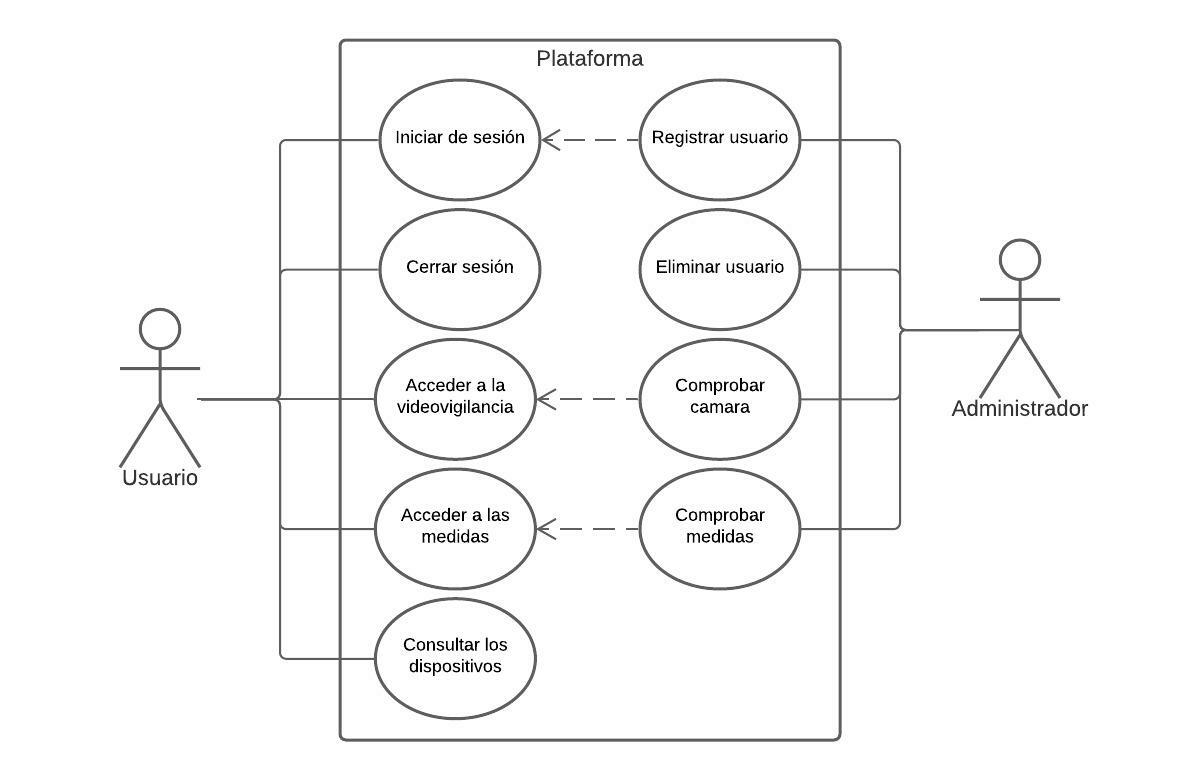
\includegraphics[scale=0.8]{casos-de-uso.jpeg}}
\end{figure}

Para realizar una descripción más detallada de los casos de uso emplearemos la representación tabular que se muestra en la siguiente plantilla.
\begin{table}[H]
	\centering
	\caption{Plantilla de los Casos de Uso}
	\begin{tabular}{|l|l|}
		\hline
		\multicolumn{2}{|c|}{\cellcolor[HTML]{BFBFBF}{\color[HTML]{000000} \textbf{CU-XX}}} \\ \hline
		\textbf{Caso de uso}     &                                                      \\ \hline
		\textbf{Actores}         &                                                      \\ \hline
		\textbf{Descripción}     &                                                      \\ \hline
		\textbf{Precondiciones}  &                                                      \\ \hline
		\textbf{Postcondiciones} & $\quad\quad\quad\quad\quad\quad\quad\quad\quad\quad$ \\ \hline
	\end{tabular}
\end{table}

\begin{itemize}
	\item \textbf{CU-XX:} Identificador del caso de uso, el XX tomará un valor en función del orden de este.
	\item \textbf{Caso de uso:} Nombre que identifica el caso de uso.
	\item \textbf{Actores:} Partes implicadas en el caso de uso.
	\item \textbf{Descripción:} Breve exposición de la situación.
	\item \textbf{Precondiciones:} Condiciones que se deben cumplir para que tenga lugar en caso de uso.
	\item \textbf{Postcondiciones:} Que ocurre si se cumple el caso de uso.
\end{itemize}

Ahora que entendemos el significado de cada una de las casillas procedemos a detallar los casos de uso.
\newcount\cu
\cu=1
\begin{table}[H]
	\centering
	\caption{CU-0\number\cu}
	\begin{tabular}{|l|l|}
		\hline
		\multicolumn{2}{|c|}{\cellcolor[HTML]{BFBFBF}{\color[HTML]{000000} \textbf{CU-0\number\cu}}} \\ \hline
		\textbf{Caso de uso}     & Registrar usuario                                          \\ \hline
		\textbf{Actores}         & Administrador                                              \\ \hline
		\textbf{Descripción}     & Crear un usuario y contraseña para acceder a la plataforma \\ \hline
		\textbf{Precondiciones}  & Acceder a la página de administración de la BBDD           \\ \hline
		\textbf{Postcondiciones} & Generación de usuario y contraseña de acceso               \\ \hline
	\end{tabular}
\end{table}
\advance\cu by 1
\begin{table}[H]
	\centering
	\caption{CU-0\number\cu}
	\begin{tabular}{|l|l|}
		\hline
		\multicolumn{2}{|c|}{\cellcolor[HTML]{BFBFBF}{\color[HTML]{000000} \textbf{CU-0\number\cu}}} \\ \hline
		\textbf{Caso de uso}     & Eliminar usuario                                 \\ \hline
		\textbf{Actores}         & Administrador                                    \\ \hline
		\textbf{Descripción}     & Revocar el acceso a la plataforma                \\ \hline
		\textbf{Precondiciones}  & Acceder a la página de administración de la BBDD \\ \hline
		\textbf{Postcondiciones} & Registro de la tabla ‘user’ eliminado            \\ \hline
	\end{tabular}
\end{table}
\advance\cu by 1
\begin{table}[H]
	\centering
	\caption{CU-0\number\cu}
	\begin{tabular}{|l|l|}
		\hline
		\multicolumn{2}{|c|}{\cellcolor[HTML]{BFBFBF}{\color[HTML]{000000} \textbf{CU-0\number\cu}}} \\ \hline
		\textbf{Caso de uso}     & Comprobar medidas                                         \\ \hline
		\textbf{Actores}         & Administrador                                             \\ \hline
		\textbf{Descripción}     & \begin{tabular}[c]{@{}l@{}}Consultar las medidas, ver que los valores sean razonables y  que\\ se reciben continuamente\end{tabular}                                \\ \hline
		\textbf{Precondiciones}  & Poseer usuario y clave de acceso de la BBDD               \\ \hline
		\textbf{Postcondiciones} & El administrador ha verificado que funciona correctamente \\ \hline
	\end{tabular}
\end{table}
\advance\cu by 1
\begin{table}[H]
	\centering
	\caption{CU-0\number\cu}
	\begin{tabular}{|l|l|}
		\hline
		\multicolumn{2}{|c|}{\cellcolor[HTML]{BFBFBF}{\color[HTML]{000000} \textbf{CU-0\number\cu}}} \\ \hline
		\textbf{Caso de uso}     & Comprobar cámara                                          \\ \hline
		\textbf{Actores}         & Administrador                                             \\ \hline
		\textbf{Descripción}     & Comprobar que la imagen de la cámara se ve y se actualiza \\ \hline
		\textbf{Precondiciones}  & Poseer usuario y clave de acceso de la web                \\ \hline
		\textbf{Postcondiciones} & El administrador ha verificado que funciona correctamente \\ \hline
	\end{tabular}
\end{table}
\advance\cu by 1
\begin{table}[H]
	\centering
	\caption{CU-0\number\cu}
	\begin{tabular}{|l|l|}
		\hline
		\multicolumn{2}{|c|}{\cellcolor[HTML]{BFBFBF}{\color[HTML]{000000} \textbf{CU-0\number\cu}}} \\ \hline
		\textbf{Caso de uso}     & Iniciar sesión                          \\ \hline
		\textbf{Actores}         & Usuario                                 \\ \hline
		\textbf{Descripción}     & Acceder a la aplicación                 \\ \hline
		\textbf{Precondiciones}  & El usuario y contraseña está registrado \\ \hline
		\textbf{Postcondiciones} & El usuario accede a la plataforma       \\ \hline
	\end{tabular}
\end{table}
\advance\cu by 1
\begin{table}[H]
	\centering
	\caption{CU-0\number\cu}
	\begin{tabular}{|l|l|}
		\hline
		\multicolumn{2}{|c|}{\cellcolor[HTML]{BFBFBF}{\color[HTML]{000000} \textbf{CU-0\number\cu}}} \\ \hline
		\textbf{Caso de uso}     & Cerrar sesión                                                   \\ \hline
		\textbf{Actores}         & Usuario                                                         \\ \hline
		\textbf{Descripción}     & El usuario termina de consultar las medidas y sale de su cuenta \\ \hline
		\textbf{Precondiciones}  & El usuario ha iniciado sesión                                   \\ \hline
		\textbf{Postcondiciones} & El usuario vuelve a la pantalla de inicio de sesión             \\ \hline
	\end{tabular}
\end{table}
\advance\cu by 1
\begin{table}[H]
	\centering
	\caption{CU-0\number\cu}
	\begin{tabular}{|l|l|}
		\hline
		\multicolumn{2}{|c|}{\cellcolor[HTML]{BFBFBF}{\color[HTML]{000000} \textbf{CU-0\number\cu}}} \\ \hline
		\textbf{Caso de uso}     & Consultar los dispositivos                                \\ \hline
		\textbf{Actores}         & Usuario                                                   \\ \hline
		\textbf{Descripción}     & Visualizar los diferentes dispositivos conectados         \\ \hline
		\textbf{Precondiciones}  & El usuario ha iniciado sesión                             \\ \hline
		\textbf{Postcondiciones} & El usuario visualiza los dispositivos, su estado y nombre \\ \hline
	\end{tabular}
\end{table}
\advance\cu by 1
\begin{table}[H]
	\centering
	\caption{CU-0\number\cu}
	\begin{tabular}{|l|l|}
		\hline
		\multicolumn{2}{|c|}{\cellcolor[HTML]{BFBFBF}{\color[HTML]{000000} \textbf{CU-0\number\cu}}} \\ \hline
		\textbf{Caso de uso}     & Acceder a las medidas                                       \\ \hline
		\textbf{Actores}         & Usuario                                                     \\ \hline
		\textbf{Descripción}     & Consultar las diferentes medidas tomadas por el dispositivo \\ \hline
		\textbf{Precondiciones}  & El usuario ha iniciado sesión y selecciona un dispositivo   \\ \hline
		\textbf{Postcondiciones} & \begin{tabular}[c]{@{}l@{}}El usuario accede a una página con las gráficas de las\\ medidas y la tabla de histórico de medidas\end{tabular}                                  \\ \hline
	\end{tabular}
\end{table}
\advance\cu by 1
\begin{table}[H]
	\centering
	\caption{CU-0\number\cu}
	\begin{tabular}{|l|l|}
		\hline
		\multicolumn{2}{|c|}{\cellcolor[HTML]{BFBFBF}{\color[HTML]{000000} \textbf{CU-0\number\cu}}} \\ \hline
		\textbf{Caso de uso}     & Acceder a la videovigilancia                              \\ \hline
		\textbf{Actores}         & Usuario                                                   \\ \hline
		\textbf{Descripción}     & Consultar la imagen de la cámara                          \\ \hline
		\textbf{Precondiciones}  & El usuario ha iniciado sesión y selecciona un dispositivo \\ \hline
		\textbf{Postcondiciones} & \begin{tabular}[c]{@{}l@{}}El usuario accede a una página con la imagen de la\\ cámara a tiempo real\end{tabular}                                \\ \hline
	\end{tabular}
\end{table}

\section{Requisitos de software}
Los requisitos descritos en esta sección se basan en los requisitos de usuario proporcionados por el cliente y los casos de uso asociados al sistema. La plantilla que se seguirá será la siguiente:
\begin{table}[H]
	\caption{Plantilla de los Requisitos Funcionales y No funcionales}
	\begin{tabular}{|l|l|}
		\hline
		\multicolumn{2}{|c|}{\cellcolor[HTML]{BFBFBF}{\color[HTML]{000000} \textbf{ID-XX}}} \\ \hline
		\textbf{Nombre}      &                                                      \\ \hline
		\textbf{Descripción} & $\quad\quad\quad\quad\quad\quad\quad\quad\quad\quad$ \\ \hline
		\textbf{Prioridad}   &                                                      \\ \hline
		\textbf{Necesidad}   &                                                      \\ \hline
		\textbf{Fuente}      &                                                      \\ \hline
		\textbf{Versión}     &                                                      \\ \hline
	\end{tabular}
\end{table}
\begin{itemize}
	\item \textbf{ID-XX:} Identifica los requisitos mediante la siguiente codificación: ID será RF si es un requisito funcional o RN si es un requisito no funcional, y XX tomará un valor en función de la posición.
	\item \textbf{Nombre:} Nombre representativo del asunto del requisito.
	\item \textbf{Descripción:} Exposición más detallada del requisito.
	\item \textbf{Prioridad:} Indica si debe ser considerado desde el principio o si por el contrario puede retrasarse. Puede ser: Alta, Mediana o Baja.
	\item \textbf{Necesidad:} Importancia del requisito sobre el sistema, pudiendo ser: Esencia, Deseable u Opcional.
	\item \textbf{Fuente:} Procedencia del requisito.
	\item \textbf{Versión:} Indica si ha sufrido variaciones a lo largo del tiempo.
\end{itemize}

Tras esta explicación de la plantilla en las siguientes subsecciones se presentan los requisitos funcionales y no funcionales.
\subsection{Requisitos Funcionales}
\newcount\rf
\rf=1
\begin{table}[H]
	\caption{RF-0\number\rf}
	\begin{tabular}{|l|l|}
		\hline
		\multicolumn{2}{|c|}{\cellcolor[HTML]{BFBFBF}{\color[HTML]{000000} \textbf{RF-0\number\rf}}} \\ \hline
		\textbf{Nombre}      & Datos de dispositivo       \\ \hline
		\textbf{Descripción} & \begin{tabular}[c]{@{}l@{}}En la lista de dispositivos el usuario podrá ver su nombre,\\ estado, última cambio de estado y un botón para acceder\\ a este\end{tabular} \\ \hline
		\textbf{Prioridad}   &                            \\ \hline
		\textbf{Necesidad}   &                            \\ \hline
		\textbf{Fuente}      & Cliente                    \\ \hline
		\textbf{Versión}     & 1.0                        \\ \hline
	\end{tabular}
\end{table}
\advance\rf by 1
\begin{table}[H]
	\caption{RF-0\number\rf}
	\begin{tabular}{|l|l|}
		\hline
		\multicolumn{2}{|c|}{\cellcolor[HTML]{BFBFBF}{\color[HTML]{000000} \textbf{RF-0\number\rf}}} \\ \hline
		\textbf{Nombre}      & Botón cerrar sesión        \\ \hline
		\textbf{Descripción} & \begin{tabular}[c]{@{}l@{}}En la parte inferior de todas las páginas aparecerá el botón\\ ‘Cerrar sesión’ que devolverá al usuario a la página de inicio\\ de sesión\end{tabular} \\ \hline
		\textbf{Prioridad}   &                            \\ \hline
		\textbf{Necesidad}   &                            \\ \hline
		\textbf{Fuente}      & Cliente                    \\ \hline
		\textbf{Versión}     & 1.0                        \\ \hline
	\end{tabular}
\end{table}
\advance\rf by 1
\begin{table}[H]
	\caption{RF-0\number\rf}
	\begin{tabular}{|l|l|}
		\hline
		\multicolumn{2}{|c|}{\cellcolor[HTML]{BFBFBF}{\color[HTML]{000000} \textbf{RF-0\number\rf}}} \\ \hline
		\textbf{Nombre}      & Botón volver               \\ \hline
		\textbf{Descripción} & \begin{tabular}[c]{@{}l@{}}Cuando se está en una página de dispositivo debe poderse\\ volver a la lista de dispositivos mediante un botón ‘Volver’\\ que se distribuyen a lo largo de la página\end{tabular} \\ \hline
		\textbf{Prioridad}   &                            \\ \hline
		\textbf{Necesidad}   &                            \\ \hline
		\textbf{Fuente}      & Cliente                    \\ \hline
		\textbf{Versión}     & 1.0                        \\ \hline
	\end{tabular}
\end{table}
\advance\rf by 1
\begin{table}[H]
	\caption{RF-0\number\rf}
	\begin{tabular}{|l|l|}
		\hline
		\multicolumn{2}{|c|}{\cellcolor[HTML]{BFBFBF}{\color[HTML]{000000} \textbf{RF-0\number\rf}}} \\ \hline
		\textbf{Nombre}      & Medidas tomadas            \\ \hline
		\textbf{Descripción} & \begin{tabular}[c]{@{}l@{}}Los datos que tome el dispositivo deben mostrarse en varios\\ formatos, uno tabular los datos concretos y otro gráfico para\\ ver la progresión de una manera más visual\end{tabular} \\ \hline
		\textbf{Prioridad}   &                            \\ \hline
		\textbf{Necesidad}   &                            \\ \hline
		\textbf{Fuente}      & Cliente                    \\ \hline
		\textbf{Versión}     & 1.0                        \\ \hline
	\end{tabular}
\end{table}

\subsection{Requisitos No Funcionales}
\newcount\rn
\rn=1
\begin{table}[H]
	\caption{RN-0\number\rn}
	\begin{tabular}{|l|l|}
		\hline
		\multicolumn{2}{|c|}{\cellcolor[HTML]{BFBFBF}{\color[HTML]{000000} \textbf{RN-0\number\rn}}} \\ \hline
		\textbf{Nombre}      &          \\ \hline
		\textbf{Descripción} &          \\ \hline
		\textbf{Prioridad}   &          \\ \hline
		\textbf{Necesidad}   &          \\ \hline
		\textbf{Fuente}      & Analista \\ \hline
		\textbf{Versión}     & 1.0      \\ \hline
	\end{tabular}
\end{table}
\advance\rn by 1


\section{Matriz de trazabilidad}